% !TEX root = ../multi_task.tex

\subsection{MultiMNIST}
We use the MultiMNIST dataset, which overlays multiple images together \citep{multi_mnist}. For each image, a different one is chosen uniformly in random. One of these images is placed at the top-left and the other at the bottom-right. We show sample MultiMNIST images in Figure~\ref{fig:sample_multi_mnist}.

\begin{figure}[ht]
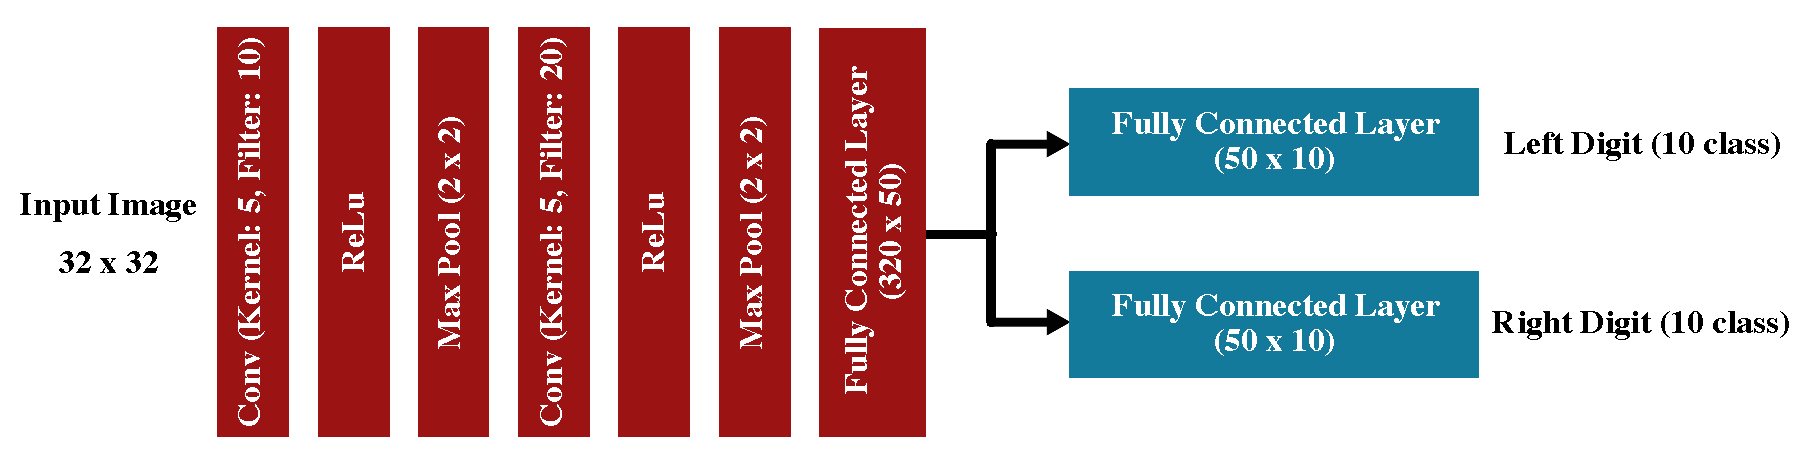
\includegraphics[width=\textwidth]{arch_multi_mnist}
\caption{Architecture used for MultiMNIST experiments.}
\label{fig:multi_mnist}
\end{figure}

\begin{figure}[hb]
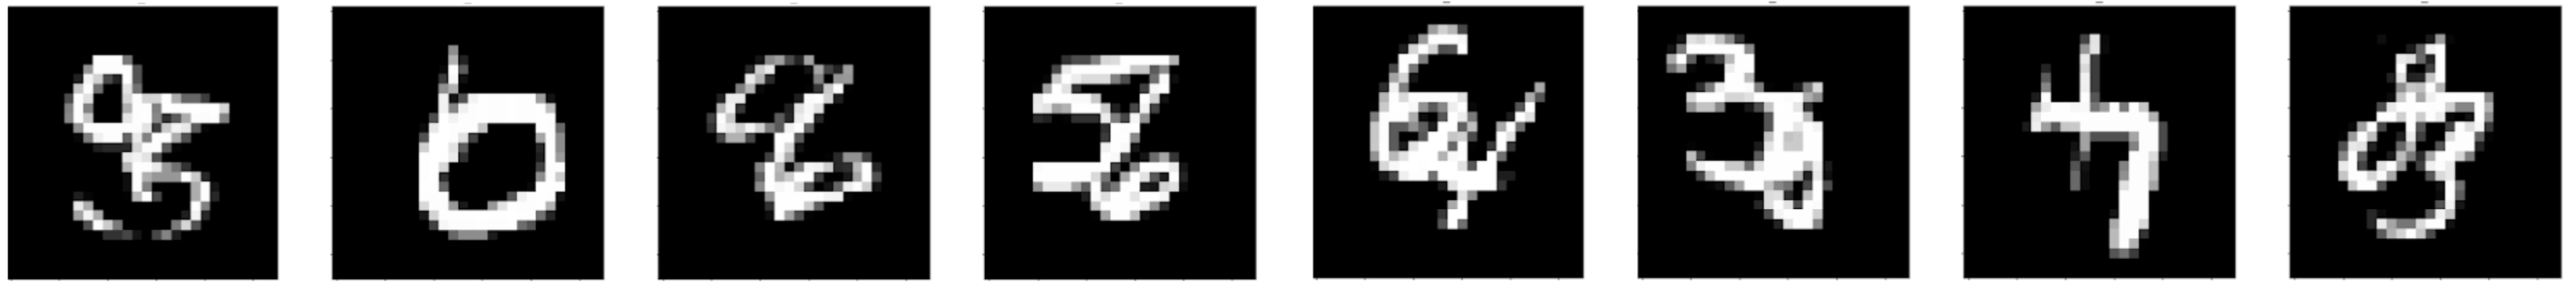
\includegraphics[width=\textwidth]{multi_mnist_vis_}
\caption{Sample MultiMNIST images. In each image, one task (task-L) is classifying the digit on the top-left and the second task (task-R) is classifying the digit on the bottom-right.}
\label{fig:sample_multi_mnist}
\end{figure}

For the MultiMNIST experiments, we use an architecture based on LeNet~\citep{mnist}. We use all layers except the final one as a shared encoder. We use the fully-connected layer as a task-specific function for the left and right tasks by simply adding two independent fully-connected layers, each taking the output of the shared encoder as input. As a task-specific loss function, we use the cross-entropy loss with a softmax for both tasks. The architecture is visualized in Figure~\ref{fig:multi_mnist}.

The implementation uses PyTorch \citep{pytorch}. For all baselines, we searched over the set $LR=\{\num{1e-4}, \num{5e-4}, \num{1e-3}, \num{5e-3}, \num{1e-2}, \num{5e-2}\}$ of learning rates and chose the model with the highest validation accuracy. We used SGD with momentum, halving the learning rate every 30 epochs. We use batch size $256$ and train for $100$ epochs. We report test accuracy.

\subsection{Multi-label classification}
For multi-label classification experiments, we use ResNet-18 \citep{resnet} without the final layer as a shared representation function. Since there are 40 attributes, we add 40 separate $2048\times2$ dimensional fully-connected layers as task-specific functions. The final two-dimensional output is passed through a 2-class softmax to get binary attribute classification probabilities. We use cross-entropy as a task-specific loss. The architecture is visualized in Figure~\ref{fig:arch_multi_label}.

The implementation uses PyTorch \citep{pytorch}. We resize each CelebA image \citep{celeba} to $64\times64\times3$. For all experiments, we searched over the set $LR=\{\num{1e-4}, \num{5e-4}, \num{1e-3}, \num{5e-3}, \num{1e-2}, \num{5e-2}\}$ of learning rates and chose the model with the highest validation accuracy. We used SGD with momentum, halving the learning rate every 30 epochs. We use batch size $256$ and train for $100$ epochs. We report attribute-wise binary accuracies on the test set as well as the average accuracy.

\begin{figure}[ht]
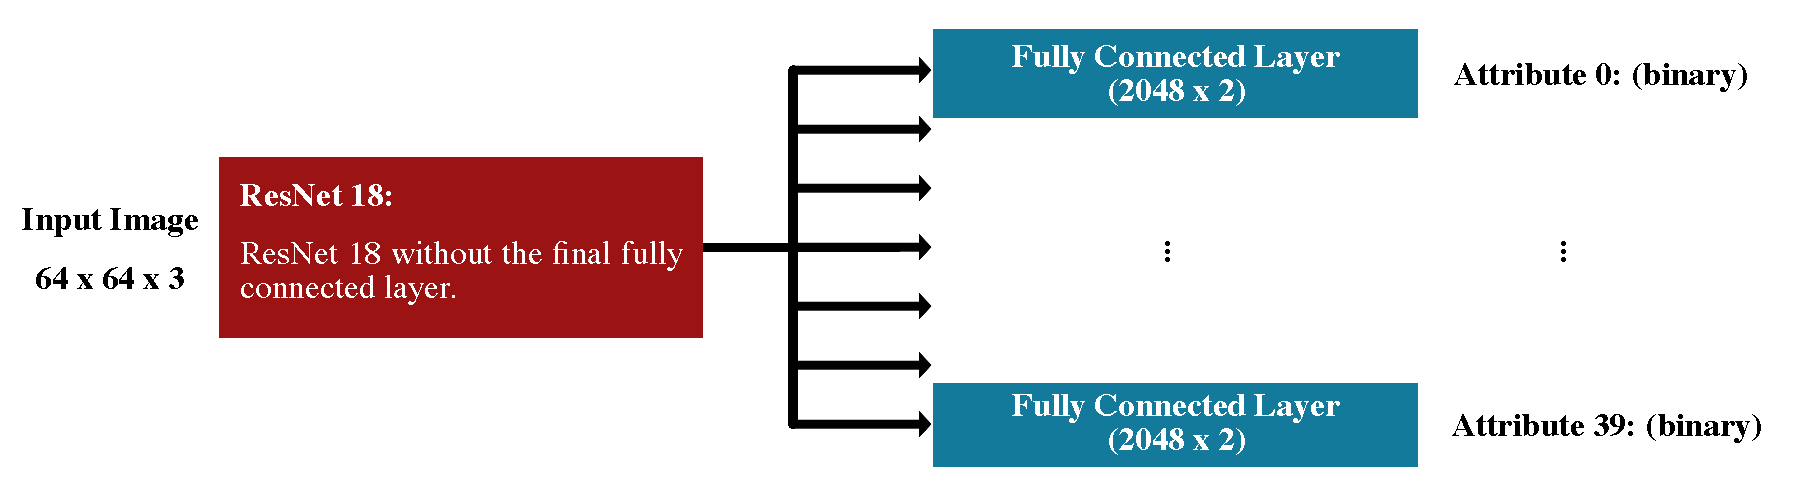
\includegraphics[width=\textwidth]{arch_multi_label}
\caption{Architecture used for multi-label classification experiments.}
\label{fig:arch_multi_label}
\end{figure}

\subsection{Scene understanding}
For scene understanding experiments, we use the Cityscapes dataset \citep{cityscapes}. We resize all images to resolution $256\times512$ for computational efficiency. As a shared representation function (encoder), we use the ResNet-50 architecture \citep{resnet} in fully-convolutional fashion. We take the ResNet-50 architecture and only use layers prior to average pooling that are fully convolutional. As a decoder, we use the pyramid pooling module \citep{pspnet} and set the output sizes to $256\times512\times19$ for semantic segmentation ($19$ classes), $256\times512\times2$ for instance segmentation (one output channel for the x-offset of the center location and another channel for the y-offset), and $256\times512\times1$ for monocular depth estimation. For instance segmentation, we use the proxy task of estimating the offset for the center location of the instance that encompasses the pixel. We directly estimate disparity instead of depth and later convert it to depth using the provided camera intrinsics. As a loss function, we use cross-entropy with a softmax for semantic segmentation, and MSE for depth and instance segmentation. We visualize the architecture in Figure~\ref{fig:scene}.

We initialize the encoder with a model pretrained on ImageNet \citep{imagenet}. We use the implementation of the pyramidal pooling network with bilinear interpolation shared by \citet{pspnet_implementation}. Ground-truth results for the Cityscapes test set are not publicly available. Therefore, we report numbers on the validation set. As a validation set for hyperparameter search, we randomly choose $275$ images from the training set. After the best hyperparameters are chosen, we retrain with the full training set and report the metrics on the Cityscapes validation set, which our algorithm never sees during training or hyperparameter search. As metrics, we use mean intersection over union (mIoU) for semantic segmentation, MSE for instance segmentation, and MSE for disparities (depth estimation). We directly report the metric in the proxy task for instance segmentation instead of performing a further clustering operation. For all experiments, we searched over the set $LR=\{\num{1e-4}, \num{5e-4}, \num{1e-3}, \num{5e-3}, \num{1e-2}, \num{5e-2}\}$ of learning rates and chose the model with the highest validation accuracy. We used SGD with momentum, halving the learning rate every 30 epochs. We use batch size $8$ and train for $250$ epochs.

\begin{figure}[ht]
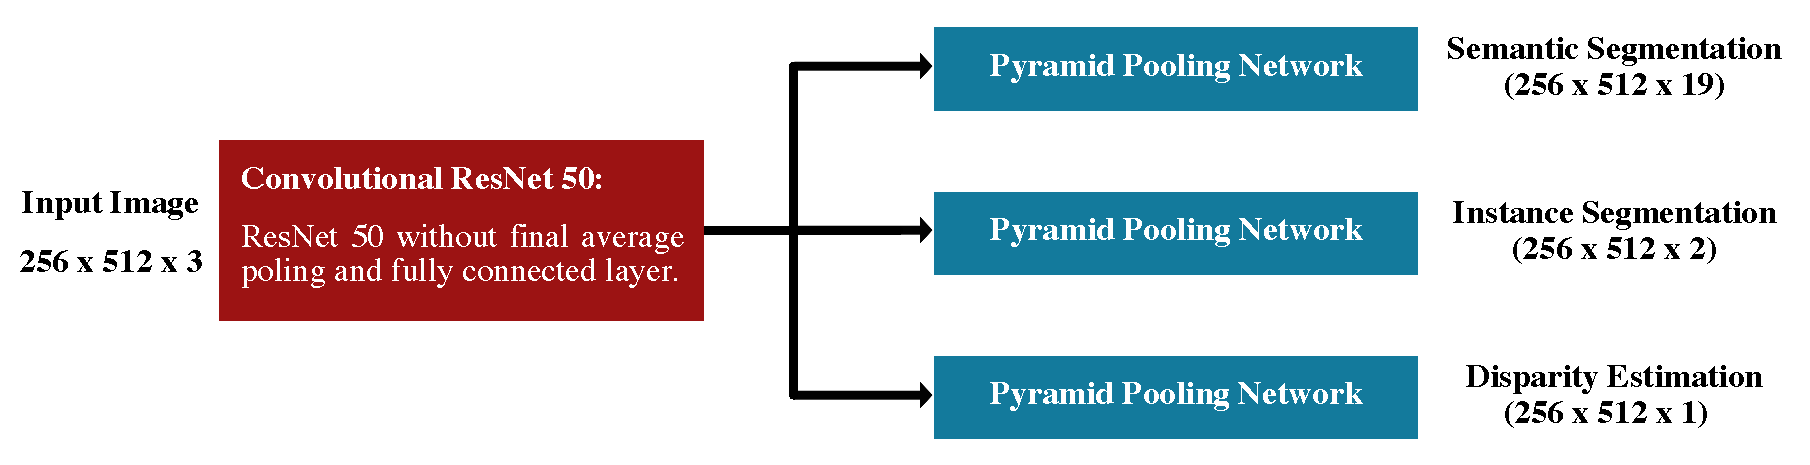
\includegraphics[width=\textwidth]{arch_cityscapes}
\caption{Architecture used for scene understanding experiments.}
\label{fig:scene}
\end{figure}
